\documentclass[11pt,a4paper]{article}
\usepackage{fontspec}\usepackage{unicode-math}\usepackage[british]{babel}
\setmainfont{Libertinus Serif}[Numbers={OldStyle,Proportional},SmallCapsFeatures={LetterSpace=6}]
\setsansfont{Libertinus Sans}\setmathfont{Libertinus Math}
\newfontfamily\tabfigs{Libertinus Serif}[Numbers={Lining,Monospaced}]
\usepackage[protrusion=true,expansion=false]{microtype}
\usepackage[a4paper,textwidth=30pc,top=28mm,bottom=30mm,hmarginratio=1:1,headsep=10mm]{geometry}
\linespread{1.08}\setlength{\parindent}{1.2em}\frenchspacing
\clubpenalty=10000 \widowpenalty=10000
\renewcommand{\topfraction}{0.85}\renewcommand{\textfraction}{0.12}\renewcommand{\floatpagefraction}{0.8}
\usepackage{xcolor}\definecolor{accent}{HTML}{2A5FA8}\definecolor{quiet}{HTML}{6B6A66}
\usepackage[explicit]{titlesec}
\titleformat{\section}{\normalfont\large}{\textcolor{accent}{\thesection}}{0.8em}{\scshape\MakeLowercase{#1}}
\titlespacing*{\section}{0pt}{2.2ex plus .5ex minus .2ex}{1.0ex}
\usepackage{fancyhdr}\pagestyle{fancy}\fancyhf{}\renewcommand{\headrulewidth}{0pt}
\fancyhead[C]{\footnotesize\scshape\textcolor{quiet}{beam shaping against systematic risk}}
\fancyfoot[C]{\footnotesize\textcolor{quiet}{\thepage}}
\usepackage{graphicx,booktabs,tabularx,multirow,array}
\usepackage[font={small,sf},labelfont={sf,color=accent},labelsep=period,justification=raggedright,singlelinecheck=false]{caption}
\captionsetup[table]{position=top,skip=4pt}
\usepackage{siunitx}
\sisetup{group-minimum-digits=5,group-separator={\,},range-phrase={--},per-mode=symbol}
\DeclareSIUnit\jansky{Jy}\DeclareSIUnit\beam{beam}\DeclareSIUnit\deg{deg}
\usepackage[style=british]{csquotes}
\usepackage[authoryear,round,sort]{natbib}\setcitestyle{aysep={},yysep={,}}
\setlength{\bibsep}{1pt}\renewcommand{\bibfont}{\small}
\usepackage[hidelinks]{hyperref}
\newcommand{\AAstar}{AA\kern0.05em$^{*}$}
\newcolumntype{L}{>{\raggedright\arraybackslash}X}

\begin{document}

\begin{center}
{\fontsize{19}{23}\selectfont Beam apodization and beamforming\\[2pt] against the AASKAII systematic risks}\par\vspace{8pt}
{\scshape answers from the aaskaii atlas risk register}\par\vspace{4pt}
{\small\textcolor{quiet}{9 November 2026}}
\end{center}
\vspace{6pt}
\begin{center}\begin{minipage}{0.9\textwidth}\small
The AASKAII Atlas risk register counts how often 16 engineering and calibration risks appear in the chapters of \emph{Advancing Astrophysics with the SKA~II}. Radio frequency interference (40 chapters), dynamic range (33) and survey speed (18) lead the list. Of the 16, beam shaping is a direct remedy for three (beam sidelobes, the primary-beam model and survey speed) and a partial remedy for eleven more; it does little for timing and nothing for the machine-learning gap between simulations and real data. SKA-Low is where the lever is strongest, because every one of the 256 antennas in a station is digitized and can carry its own complex, frequency-dependent weight. A toy model of an SKA-Low station shows the price. A 28 dB Taylor taper lowers the first sidelobe from −17 to −27 dB for an efficiency of 0.85, which is a 39\% increase in observing time. A frequency-scaled taper that holds the beam fixed between 120 and 180 MHz cuts main-lobe chromaticity from 5 dB to under 1 dB, but its efficiency falls to 0.42 at the top of the band. Spatial nulls toward three interferers cost almost nothing in gain, and calibration errors of 1--5\% in element gain still leave 31--17 dB of suppression. At \AAstar, with 307 stations and 60\% of the AA4 array gain, these costs fall on a telescope that already needs roughly 2.8 times the AA4 integration time, so apodization should be applied selectively, by project.
\end{minipage}\end{center}
\vspace{4pt}

\section{The register and what beamforming can reach}

The AASKAII Atlas (version 2, generated 4 October 2026) searches every chapter of the 2026 science book for 16 named risks and counts a chapter only when it names a risk at least twice. The counts measure how widely a risk is discussed, not how severe it is, and the register says as much. Figure~\ref{fig:register} shows them, coloured by how far beam shaping could answer each risk, and Table~\ref{tab:summary} sets out the reasoning behind each judgement.

\begin{figure}[!htb]
\centering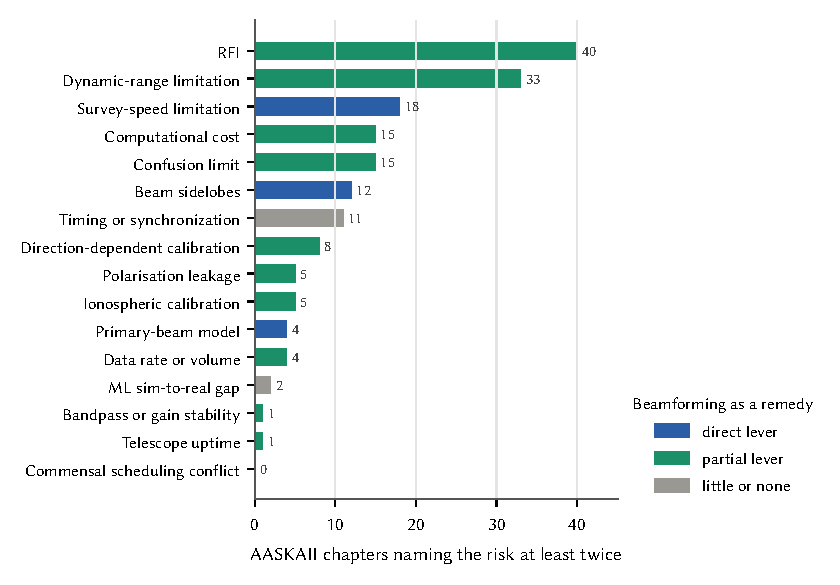
\includegraphics[width=0.8\textwidth]{fig_register.pdf}
\caption{The 16 risks of the AASKAII Atlas register, ranked by the number of chapters that name each at least twice. Colour gives this report's judgement of whether station apodization, null-steering or tied-array beamforming offers a direct remedy, a partial one, or little or none.}
\label{fig:register}
\end{figure}

Two kinds of beamforming matter. The first is the station beamformer of SKA-Low, which sums the signals of 256 dual-polarized log-periodic antennas spread over a station about \SI{38}{\metre} across. Because each antenna is digitized, the weights can be chosen freely: tapered to shape the beam, made frequency-dependent, restricted to a subset of antennas to form substations, or duplicated to point several beams at once \citep{Trott2026,Trott2024}. Apodization is the name the SKA community gives to this weighting \citep{Trott2026,Datta2026}. The second kind is the tied-array beam, which sums stations or dishes coherently. At \AAstar\ the pulsar search system offers 250 tied-array beams for SKA-Low and 1125 for SKA-Mid, against 500 and 1500 at AA4; the timing system offers 16 voltage beams \citep{Keane2026}; VLBI uses at least four independently steerable beams formed from a core subarray \citep{SKAO2021}. SKA-Mid dishes have fixed primary beams, so apodization in the sense used here is an SKA-Low capability, and SKA-Mid shares only the tied-array part of the story.

\section{Apodization against sidelobes and beam-model error}

Twelve chapters name beam sidelobes and four name the primary-beam model. The concern is the same in each: sources outside the main lobe leak into the data through sidelobes that are poorly modelled and change with frequency. At low frequencies this leakage behaves like an extra noise term. \citet{Mort2017}, cited by \citet{Tripathi2026} and \citet{Datta2026}, called it far-sidelobe source noise and found in simulations that it may limit SKA-Low sensitivity in observations longer than about 12 hours; for unapodized stations at 50 MHz the thermal noise reached the far-sidelobe level after roughly 27 hours. In image-plane transient searches the same sidelobes create false candidates around bright sources \citep{Andersson2026}.

\citet{Trott2026} show Gaussian tapers at 100 MHz and draw the rule that matters most: apodization smooths the beam and lowers the inner sidelobes, but it does not change the outer sidelobes, which are set by the discrete positions of the antennas. A toy model reproduces both halves of that rule (Figure~\ref{fig:beams}, Table~\ref{tab:tapers}). With uniform weights the first sidelobe sits at −17 dB. A Gaussian taper with a width equal to the station radius lowers it to −19 dB for an efficiency of 0.98; a 28 dB Taylor taper lowers it to −27 dB for an efficiency of 0.85; a Gaussian half as wide lowers it to −30 dB for 0.75. The Taylor case agrees with \citet{Mort2017}, who found that a 28 dB Taylor taper cost about 15\% in sensitivity and halved the far-sidelobe source noise at low frequencies.

\begin{figure}[!htb]
\centering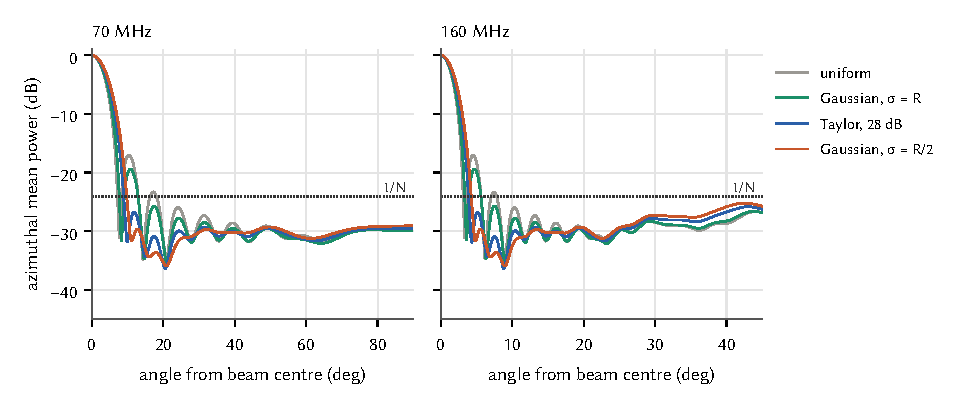
\includegraphics[width=\textwidth]{fig_beams.pdf}
\caption{Azimuthally averaged power of a model SKA-Low station beam at zenith for four weightings. Tapering lowers the first sidelobes and widens the main lobe. At 160 MHz the far sidelobes settle near the random-array floor of $1/(N\eta)$, which rises slightly as the taper strengthens; at 70 MHz, where the antennas are closely packed, they lie below it.}
\label{fig:beams}
\end{figure}

Beyond the first few sidelobes the picture changes. Above about 100 MHz the antennas are sparse in wavelengths, the far sidelobes behave like those of a random array, and their mean power is $1/(N\eta)$ for $N$ antennas and taper efficiency $\eta$. For 256 antennas this floor is −24 dB, and a taper raises it slightly, by 0.7 dB for the Taylor case. Apodization therefore trades lower near-in sidelobes for a marginally higher far-sidelobe floor. The far sidelobes can only be lowered by more antennas per station, by averaging over stations with different rotations or layouts, or by modelling and subtracting the bright sources they admit, as \citet{Pober2016} showed for wide-field foregrounds in early MWA data \citep[cited in][]{Burba2026}.

\begin{table}[!htb]
\caption{Metrics of the model station beam at 160 MHz. Efficiency $\eta$ is the loss in signal-to-noise ratio; the time factor $1/\eta^{2}$ is the extra integration needed to recover it.}
\label{tab:tapers}
\centering\small\tabfigs
\begin{tabular}{@{}lccccc@{}}
\toprule
Weighting & FWHM & First sidelobe & Far floor & $\eta$ & Time\\
 & (deg) & (dB) & (dB) & & factor\\
\midrule
Uniform & 2.84 & −17.0 & −24.5 & 1.00 & 1.00\\
Gaussian, $\sigma=R$ & 2.97 & −19.4 & −24.5 & 0.98 & 1.05\\
Taylor, 28 dB & 3.27 & −26.8 & −23.9 & 0.85 & 1.39\\
Gaussian, $\sigma=R/2$ & 3.48 & −29.7 & −23.3 & 0.75 & 1.79\\
\bottomrule
\end{tabular}
\end{table}

The more important gain is in the model. A tapered beam has a broad, smooth main lobe and inner sidelobes that change slowly with direction and frequency, which makes it easier to fit with a small number of parameters and less sensitive to the loss of individual antennas. \citet{Burba2026} note that faulty elements and mutual coupling make dipole-array beams complex and unstable; reweighting the surviving antennas to restore a symmetric taper is one way to recover a predictable beam when elements fail. It does not remove the effects of mutual coupling, which alter each antenna's embedded pattern. \citet{deLeraAcedo2026}, summarizing \citet{OHara2025}, report that beam models built from averaged embedded patterns leave residuals of about 1\% in 21 cm power spectra, several orders of magnitude above the signal, and that beams may need to be known to four or five significant figures. Apodization reduces how much of that accuracy the analysis depends on; it cannot supply the accuracy itself.

\section{Achromatic beams for the 21 cm window}

For the epoch of reionization the risk is spectral rather than spatial. Sidelobe structure that changes with frequency imparts spectral structure to residual foregrounds and leaks power into the region of Fourier space where the 21 cm signal should be clean \citep{Trott2026}. \citet{Trott2026} identify frequency-dependent complex weights as the most flexible remedy, able to make the beam spectrally achromatic over part of the sky, and list apodization alongside substations and multi-beaming among the telescope features the science working group will rely on.

The toy model shows how much a simple version achieves (Figure~\ref{fig:chrom}). A Gaussian taper whose width scales with wavelength holds the main lobe fixed at its 120 MHz size. Over 120--180 MHz the beam power two degrees from the centre varies by 0.8 dB, against 5.1 dB for uniform weights; four degrees out it varies by 2.5 dB against 14 dB, where the uniform beam passes through its first null. In one fixed direction twenty degrees out, the spread falls from 47 dB to 10 dB. The cost rises steeply with frequency, because the taper must narrow to keep the beam fixed: the efficiency is 0.75 at 120 MHz, 0.57 at 150 MHz and 0.42 at 180 MHz. A 21 cm experiment would therefore use achromatic weights over a limited band, or accept a beam that is achromatic only in the main lobe, where calibration is most accurate.

\begin{figure}[!htb]
\centering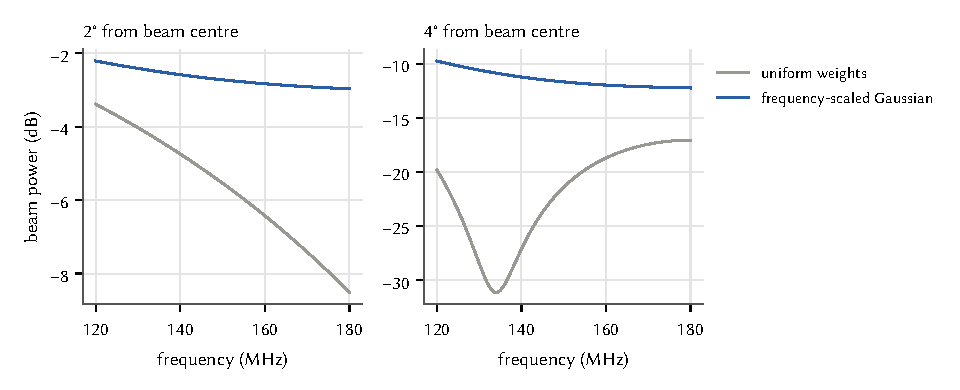
\includegraphics[width=\textwidth]{fig_chrom.pdf}
\caption{Beam power against frequency at two angles from the beam centre for the model station. A Gaussian taper whose width scales with wavelength keeps the main lobe nearly fixed; uniform weights let the beam shrink with frequency, so the response at four degrees falls through the first null near 135 MHz.}
\label{fig:chrom}
\end{figure}

\section{Spatial nulling against interference}

RFI is the most widely discussed risk in the register, named in 40 chapters across all seven sections. Most of it is handled by flagging in time and frequency, which beamforming does not replace. Part of it, however, arrives from a few known and moving directions. \citet{Keane2026} exclude 240--270 MHz from SKA-Low pulsar searches because of high-occupancy interference, and note that satellite emission appears across the whole band at least a few per cent of the time. \citet{Grigg2025} detected \num{112534} transits of \num{1806} Starlink satellites in about 76 million all-sky images from a prototype station on the SKA-Low site, with a satellite present in up to about 30\% of images in some datasets.

A digitized station can place a null on each interferer by projecting its weights away from the interferer's direction. In the toy model, three nulls at 110 MHz cost 0.014 dB of boresight gain (Figure~\ref{fig:nulls}). The depth achieved in practice is set by how well the antennas are calibrated. With random gain and phase errors of 1\% rms the median suppression relative to the unnulled sidelobe is 31 dB; at 3\% it is 22 dB, at 5\% 17 dB and at 10\% 12 dB. Because satellites move, the weights must be updated on a cadence set by the time a satellite takes to cross a null, and the nulls make the station beam time-variable, which the beam model must then follow. Spatial nulling is therefore best seen as a way to lower the interference that reaches the correlator before flagging, not as a substitute for flagging.

\begin{figure}[!htb]
\centering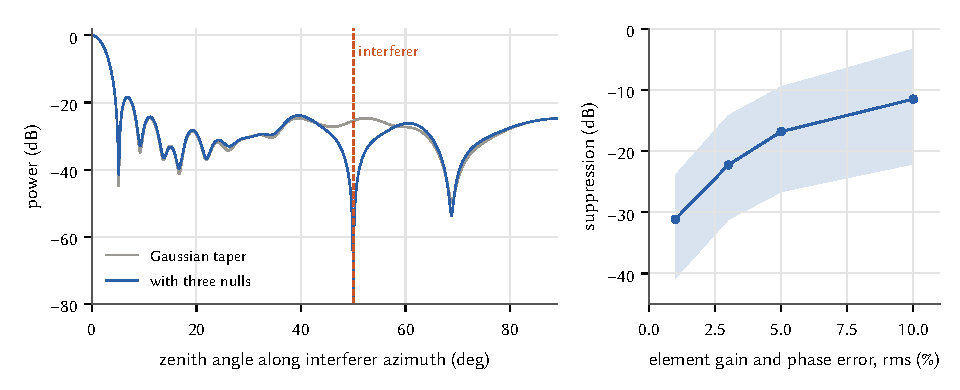
\includegraphics[width=\textwidth]{fig_nulls.pdf}
\caption{Left: a cut through the model station beam at 110 MHz before and after three nulls are placed on interferers, one of which lies 50 degrees from zenith in this cut. Right: suppression at the null directions, relative to the unnulled beam, when the antennas carry random gain and phase errors; points are medians and the band spans the 10th to 90th percentiles over 200 trials.}
\label{fig:nulls}
\end{figure}

\section{Calibration, the ionosphere and polarization}

Direction-dependent calibration (8 chapters), ionospheric calibration (5) and polarization leakage (5) are not solved by beam shaping, but each becomes easier when the beam is stable and well modelled. \citet{Datta2026} argue that apodization and substations will help SKA-Low observe the ionosphere. A full station sees three to five degrees, smaller than many ionospheric structures, so large coherent patterns appear as rapid and apparently random direction-dependent phase errors; tapering or using fewer antennas widens the field of view so those structures can be followed, at a cost in sensitivity \citep{Datta2026,Mort2017,Trott2024}. For polarization, \citet{Patra2026} trace leakage at low frequencies to differences between the modelled and true beam, which convert Stokes $I$ into $Q$, $U$ and $V$. A symmetric, smooth beam narrows that difference. For the Sun, which is the extreme case of a bright source, \citet{Oberoi2026} note that small substations dilute the solar signal and widen the field, and propose a commensal solar monitoring subarray of small substations that uses less than 0.5\% of the collecting area.

Dynamic range, named in 33 chapters, depends on all of these. Apodization helps where the limit comes from bright sources in the inner sidelobes, and null-steering can suppress a known bright source as well as an interferer, though a null that moves across the sky changes the beam in ways that peeling must then follow. Where the limit comes from calibration errors or from the synthesized beam, beam shaping does not help. The same holds for the confusion limit, named in 15 chapters: it lowers sidelobe confusion from sources outside the field, but classical confusion within the field is set by the synthesized beam and the source counts.

\begin{table}[!htb]
\caption{Where beam shaping acts on the register's risks, and its main cost or limit. Ch.\ is the number of chapters in the Atlas register that name the risk at least twice.}
\label{tab:summary}
\centering\footnotesize
\setlength{\tabcolsep}{4pt}\begin{tabularx}{\textwidth}{@{}>{\raggedright\arraybackslash}p{8.6em}>{\tabfigs}r L L@{}}
\toprule
Risk & Ch. & Lever & Cost or limit \\
\midrule
RFI & 40 & Nulls on satellites and other moving sources & Depth set by calibration; time-variable beam \\
Dynamic range & 33 & Lower inner sidelobes; nulls on bright sources & Calibration errors untouched \\
Survey speed & 18 & Tied-array tiling; several station beams & 250 search beams at \AAstar \\
Computational cost & 15 & Beam data in place of correlations & Downstream load unchanged \\
Confusion limit & 15 & Lower sidelobe confusion & Classical confusion untouched \\
Beam sidelobes & 12 & Apodization & Efficiency 0.85--0.98 for −27 to −19 dB \\
Timing & 11 & None; a prerequisite & --- \\
Direction-dependent calibration & 8 & Smooth, stable beams & Coupling remains \\
Polarization leakage & 5 & Symmetric beam, better model & Needs measured beams \\
Ionospheric calibration & 5 & Wider field via taper or substations & Sensitivity \\
Primary-beam model & 4 & Smooth, achromatic weights & Efficiency 0.42 at 180 MHz \\
Data rate & 4 & Compression by beamforming & Partial \\
ML sim-to-real gap & 2 & None & --- \\
Bandpass or gain stability & 1 & Beam only, not receivers & --- \\
Telescope uptime & 1 & Reweighting around failed antennas & Model must track faults \\
Commensal scheduling & 0 & Multi-beam and substations & Bandwidth shared \\
\bottomrule
\end{tabularx}
\end{table}

\section{Survey speed, data rate and commensality}

Survey speed is named in 18 chapters and is the risk on which tied-array beamforming acts most directly. \citet{Keane2026} choose the inner kilometre of each array for pulsar searches because the tied-array beam's field of view shrinks as the inverse square of the maximum baseline. At \AAstar\ that region holds 192 SKA-Low stations with a gain of \SI{29.5}{\kelvin\per\jansky}, against 217 stations and \SI{33.4}{\kelvin\per\jansky} at AA4; the full \AAstar\ array of 307 stations reaches \SI{47.2}{\kelvin\per\jansky}, against \SI{78.8}{\kelvin\per\jansky} for the 512 stations of AA4. The number of search beams, 250 at \AAstar\ against 500 at AA4, halves the sky that SKA-Low can tile in each pointing.

At the station level, \citet{Trott2026} note that 21 cm experiments need only 75--150 MHz of the 300 MHz bandwidth, so two to four station beams can be formed on separate fields at no cost in bandwidth they would use, trading thermal noise for sample variance. The same mechanism is the main route to commensal observing, a risk the register finds in no chapter but which the multi-beam and substation designs address directly. Beamforming also reduces data rate and computing load: a station beam compresses 256 antenna streams into one, and a tied-array beam replaces a full correlation with a time series. The register's four data-rate chapters and 15 computational-cost chapters are concerned mainly with downstream processing, so this is a partial lever only.

\section{What stays out of reach}

Three risks are untouched or made harder by beamforming. Timing and synchronization, named in 11 chapters, is a prerequisite for coherent beams rather than something they fix; the stability of the beamformer limits how large a VLBI subarray can be \citep{SKAO2021}. The gap between simulated and real data in machine-learning methods, named in two chapters, is unaffected, except that a stable, well-modelled beam narrows the difference between the simulated and real instrument. Mutual coupling between antennas and between neighbouring stations, which \citet{deLeraAcedo2026} identify as a likely limit for 21 cm work, is not removed by weighting, because the weights act on embedded patterns that already contain it. Bandpass and gain stability, named in one chapter, likewise belong to the analogue chain; frequency-dependent weights can flatten the beam but not the receivers.



\section{Recommendations for AA*}

The case for apodization is strongest where the science is limited by systematics rather than noise, and \AAstar\ makes noise dearer. With 60\% of the AA4 array gain, an \AAstar\ observation needs about 2.8 times the AA4 integration time to reach the same depth; adding a 28 dB Taylor taper raises that to about 3.9 times (an estimate; see the note on methods). For continuum and pulsar surveys, which are limited by noise or confusion, the default should be uniform or lightly tapered weights, with a Gaussian of the station radius costing only 2\% in signal-to-noise. For 21 cm power spectra, wide-field polarimetry and ionospheric studies, a moderate taper is justified, and frequency-scaled weights should be offered over sub-bands of 30--60 MHz, where their efficiency stays above about 0.5.

Four steps would make these options usable during \AAstar. The observatory could publish a small set of standard weightings, each with measured beam models, so that analyses do not have to model bespoke beams; the SKA-Low station beam simulator cited by \citet{Datta2026} is a natural home for them. It could test spatial nulling on satellites with the prototype stations, measuring the null depth achieved against the calibration accuracy of the antennas, since the toy model suggests 1--3\% accuracy is needed for 20--30 dB of suppression. It could expose substations and multiple station beams in commensal templates, building on the substation templates of \citet{Trott2024}. And it could compare apodized and unapodized beams in end-to-end simulations that include mutual coupling, because it is the coupling, not the taper, that \citet{deLeraAcedo2026} expect to set the limit.

\section*{\scshape note on methods}
\small
The station model places 256 isotropic antennas at random within a \SI{38}{\metre} circle with a minimum spacing of \SI{1.5}{\metre}, and computes the array factor only; it omits the element pattern, mutual coupling and polarization, so it shows trends rather than predicting the SKALA4.1 beam. Efficiency is $\eta=|\sum w|^{2}/(N\sum w^{2})$, and the time factor $1/\eta^{2}$ assumes that sky noise dominates and is uncorrelated between antennas. The Taylor taper is a one-dimensional Taylor window applied along the radius. Nulls are formed by projecting the weights onto the space orthogonal to the interferer steering vectors; calibration errors are independent Gaussian errors in amplitude and phase. The \AAstar\ factors use the array gains of \citet{Keane2026}: $(78.8/47.2)^{2}\approx2.8$, multiplied by 1.39 for the taper. The live SKAO sensitivity calculator was unavailable during this work, so no calculator values are quoted. The figure script, simulation code and LaTeX source accompany this report.

\normalsize
\begin{thebibliography}{99}
\bibitem[{Andersson et~al.(2026)}]{Andersson2026}
Andersson, A., Dobbie, D., Hurley-Walker, N., et~al. (2026), \enquote{Commensal Image Plane Transient Search Methods with the SKAO}, in \emph{Advancing Astrophysics with the SKA~II}.

\bibitem[{Burba et~al.(2026)}]{Burba2026}
Burba, J., Bull, P., Ceccotti, E., et~al. (2026), \enquote{Foreground Characterization and Mitigation in the Observations of the CD/EoR with the SKA}, in \emph{Advancing Astrophysics with the SKA~II}.

\bibitem[{Datta et~al.(2026)}]{Datta2026}
Datta, A., Pal, S.~K., Mangla, S., et~al. (2026), \enquote{Studying Ionosphere Using SKA-Low and SKA-Mid}, in \emph{Advancing Astrophysics with the SKA~II}.

\bibitem[{de~Lera~Acedo et~al.(2026)}]{deLeraAcedo2026}
de Lera Acedo, E., Aguirre, J., Anstey, D., et~al. (2026), \enquote{Observations of the Cosmic Dawn and Epoch of Reionization with the SKAO: Observational Lessons Learned from Precursors and Pathfinder Instruments}, in \emph{Advancing Astrophysics with the SKA~II}.

\bibitem[{Grigg et~al.(2025)}]{Grigg2025}
Grigg, D., Tingay, S., and Sokolowski, M. (2025), \enquote{The Growing Impact of Unintended Starlink Broadband Emission on Radio Astronomy in the SKA-Low Frequency Range}, arXiv:2506.02831.

\bibitem[{Keane et~al.(2026)}]{Keane2026}
Keane, E.~F., Graber, V., Levin, L., et~al. (2026), \enquote{A Square Kilometre Array Pulsar Census}, in \emph{Advancing Astrophysics with the SKA~II}.

\bibitem[{Mort et~al.(2017)}]{Mort2017}
Mort, B., Dulwich, F., Razavi-Ghods, N., de Lera Acedo, E., and Grainge, K. (2017), \enquote{Analysing the Impact of Far-out Side-lobes on the Imaging Performance of the SKA-LOW Telescope}, \emph{Monthly Notices of the Royal Astronomical Society}, 465: 3680--92.

\bibitem[{Oberoi et~al.(2026)}]{Oberoi2026}
Oberoi, D., Kansabanik, D., Mondal, S., et~al. (2026), \enquote{State-of-the-art Observation, Calibration, and Imaging Framework for Solar and Heliospheric Sciences with SKAO}, in \emph{Advancing Astrophysics with the SKA~II}.

\bibitem[{O'Hara et~al.(2025)}]{OHara2025}
O'Hara, O.~S.~D., et~al. (2025), \enquote{Uncovering the Effects of Array Mutual Coupling in 21-cm Experiments with the SKA-Low Radio Telescope}, arXiv:2412.01699.

\bibitem[{Patra et~al.(2026)}]{Patra2026}
Patra, D., Majee, P., Dey, S., et~al. (2026), \enquote{Coronal Magnetography Using Spectropolarimetry with SKA Telescopes}, in \emph{Advancing Astrophysics with the SKA~II}.

\bibitem[{Pober et~al.(2016)}]{Pober2016}
Pober, J.~C., et~al. (2016), \enquote{The Importance of Wide-field Foreground Removal for 21~cm Cosmology: A Demonstration with Early MWA Epoch of Reionization Observations}, \emph{Astrophysical Journal}, 819: 8.

\bibitem[{SKA Observatory(2021)}]{SKAO2021}
SKA Observatory (2021), \emph{SKA Observatory Establishment and Delivery Plan} (SKA Observatory).

\bibitem[{Tripathi et~al.(2026)}]{Tripathi2026}
Tripathi, P., Rivi, M., Prunet, S., Harrison, I., and Ferrari, A. (2026), \enquote{Weak Lensing with the SKAO: Radio Shear Measurement}, in \emph{Advancing Astrophysics with the SKA~II}.

\bibitem[{Trott et~al.(2024)}]{Trott2024}
Trott, C., Breen, S., Green, J., and Pearce, S. (2024), \enquote{SKA-Low Substation Templates}, Zenodo, doi:10.5281/zenodo.16951143.

\bibitem[{Trott et~al.(2026)}]{Trott2026}
Trott, C.~M., Bernardi, G., Breitman, D., et~al. (2026), \enquote{Overview of 21cm Experiments at High Redshift with SKAO}, in \emph{Advancing Astrophysics with the SKA~II}.
\end{thebibliography}

\section*{\scshape about this report}
\small
This report was prepared in Claude (Cowork), with the session configured for the model claude-sonnet-5-5 and reporting claude-opus-5-5 as the serving model; the effort level is not known. The astronomy-rag connector provided searches of AASKAII and the SKA capability documents, bibliographic look-ups and citation checks; its Google Scholar search returned nothing, and its live SKAO sensitivity calculator was unreachable. Web search confirmed the titles and abstracts of \citet{Mort2017} and \citet{Grigg2025}. The risk register was read from the AASKAII Atlas data file on the user's computer. The SKA science report skill set the form; the toolchain was XeLaTeX with Libertinus fonts, and Matplotlib with NumPy and SciPy for the station model and figures.

Up to typesetting, the session made 47 model calls, read about 10.5 million tokens (most of them from the prompt cache) and wrote about \num{43000}; weighted by cost, with cache reads at one-tenth, cache writes at twice and output at five times the input rate, this is equivalent to about 1.7 million input tokens. These figures cover the session up to typesetting.
\end{document}
